\documentclass[sigconf]{acmart}


%packages
\usepackage{listings}
\usepackage{algorithm, algpseudocode}
%\usepackage{setspace} % for \singlespacing
\usepackage{enumitem} %for \begin{itemize}[leftmargin=*]
\usepackage{subfig} % for two figures side by side
\usepackage[titletoc,title]{appendix}
%packages

\chardef\_=`_

\lstdefinestyle{redkeyword}{
	language=C,
	emptylines=1,
	breaklines=true,
	basicstyle=\ttfamily\color{black}\tiny,
	moredelim=**[is][\color{red}]{@}{@},
}

\lstdefinestyle{code}{
	language=Matlab,
	emptylines=1,
	breaklines=true,
	basicstyle=\ttfamily\color{black}\footnotesize\linespread{0.3},
	numbers=left,
	xleftmargin=2em,
	numbersep=5pt,
	stepnumber=1,
	showstringspaces=false,
	tabsize=1,
	breakatwhitespace=false,
	moredelim=**[is][\color{red}]{@}{@},
}

% this affects all the lstlisting
\begin{comment}
\lstset{
	basicstyle=\ttyfamily,
	columns=fullflexible,
	frame=single
	breaklines=true,
	postbreak=\mbox{\textcolor{red}{$\hookrightarrow$}\space},
}
\end{comment}






\fancyhf{} % Remove fancy page headers 
%\fancyhead[C]{Anonymous submission \#9999 to ACM CCS 2017} % TODO: replace 9999 with your paper number
%\fancyfoot[C]{\thepage}

\setcopyright{none} % No copyright notice required for submissions
%\acmConference[Anonymous Submission to ACM CCS 2017]{ACM Conference on Computer and Communications Security}{Due 19 May 2017}{Dallas, Texas}
%\acmYear{2017}

\settopmatter{printacmref=false, printccs=true, printfolios=true} % We want page numbers on submissions


%%\ccsPaper{9999} % TODO: replace with your paper number once obtained




\title{A Simple 8-bit CPU Implementation on FPGA \\
(Development Project)}


\author{
Zhuoyang Xiao, %\textit{(196002825)},
Haofan Zhang, %\textit{(187001615)},
Jie Ji, %\textit{(174007674)},
Mingbo Zhang %\textit{(166009308)}
}


\begin{document}

\maketitle

%! TEX root = 'main.tex'
\section{Motivation}
\label{sec:motivation}
In the computer architecture course, we learned about pipelines, branch prediction, multiple issue, reservation stations and etc. But those technologies are very complicated to implement. So we are wondering, aside from these advanced technologies, how does the simplest CPU work? What is a bus? What micro instructions are like? To answer these questions, we decide to learn a very simple CPU. We found a Youtube channel~\footnote{https://www.youtube.com/user/eaterbc} explaining how various CPU components work, and make an 8-bit CPU using TTL logic components. Because we do not have so many kinds of TTL logic components and we also want to learn about FPGA, we decided to make a similar 8-bit CPU on the FPGA development board. All the code for this project is uploaded to github~\footnote{https://github.com/whensungoesdown/8bitcpu}.

%! TEX root = 'main.tex'
\section{Team Members}
\label{sec:team}


\begin{itemize}
	\item Zhuoyang Xiao (196002825)
	\item Haofan Zhang (187001615)
	\item Jie Ji (174007674)
	\item Mingbo Zhang (166009308)
\end{itemize}


The individual tasks assigned to each group member are as follows:

Zhuoyang Xiao: 8-bit register including IR, MAR and general registers.

Haofan Zhang: 8-bit counter for PC and micro-instruction counter.

Jie Ji: RAM and ROM.

Mingbo Zhang: Control logic and module assembly.

%! TEX root = 'main.tex'
\section{Design}
\label{sec:design}
In this section, we introduce the overall design and each major components in this toy CPU.

\subsection{Design Specification}
To make the design simple enough so that we can fully understand, 8-bit processor seems to be a good choice. Because a byte has 8 bits, a 4-bit processor can be cumbersome when reading/writing memory. It needs to read/write the memory twice for one byte, and the 4-bit register cannot store the entire byte. After deciding the processor is 8-bit, next, we want to make a 8-bit, fixed length instruction set. It's much easier to decode and to fetch instructions compares to variable length instruction set as in x86 architecture.

The following is our design specification, based on the 8-bit setting.

\begin{itemize}
	\item 8-bit instruction
	\item 8-bit general register
	\item 4-bit memory address
	\item Shared 4-bit address bus and 8-bit data bus (share 8 lines)
	\item Control signals (control bus)
\end{itemize}

The CPU has one 4-bit program counter (PC), one 8-bit instruction register (IR), two 8-bit general register, one arithmetic logic unit (ALU), one memory address register (MAR), one output register and 16-byte static memory (SRAM). These components are all connected to an 8-bit bus. It also has a control logic module that issues control signals to all the components. The overall view of the CPU's schematic is shown in~\autoref{fig:cpu}.  

\begin{figure}[th]
	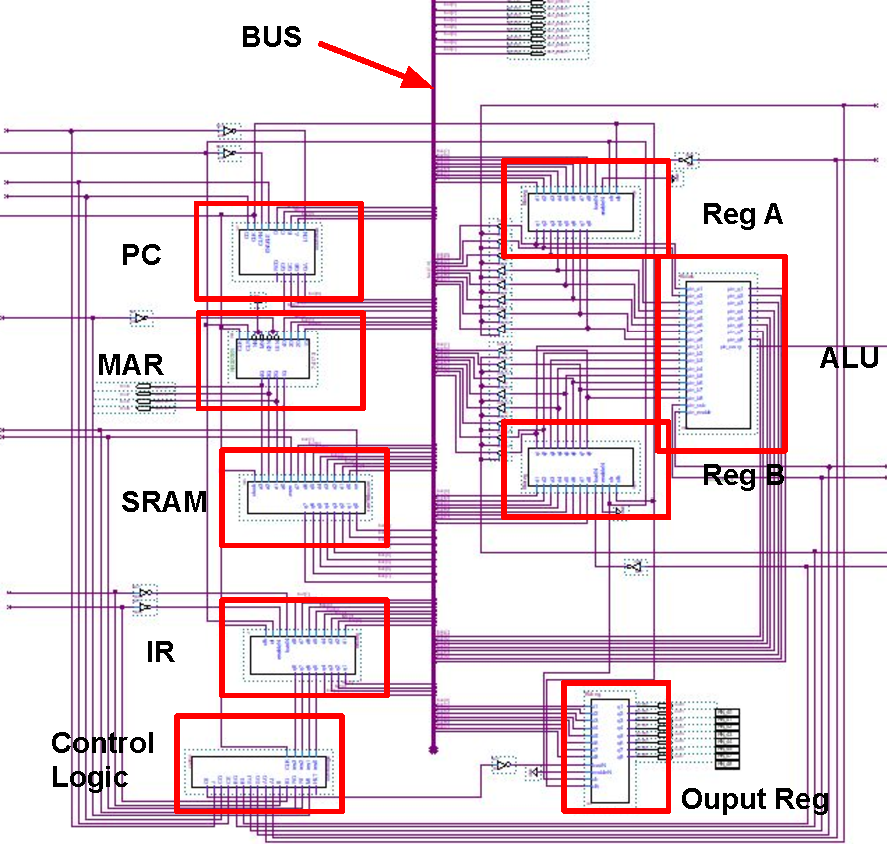
\includegraphics[width=0.47\textwidth]{figures/cpu}
	\centering
	\caption{The overall view of the CPU}
	\label{fig:cpu}
\end{figure}

The thick line in the middle is the bus which has 8 lines. It transfers both address and data. All the component connects to the bus, that is, all components can be connected to each other through the bus. And this is achieved through the control logic module. We will explain it in more detail in the following sections.


\subsection{Instruction Set}

Now we can create instruction set by ourselves. First we have to determine the format of the instruction. The upper 4-bit is opcode. All instructions have at most one operand, and this operand is a 4-bit memory address, as shown in~\autoref{fig:opcode}. There is no register operand, so some instructions have a default register. This design also leads us to only one memory addressing mode.

\begin{figure}[th]
	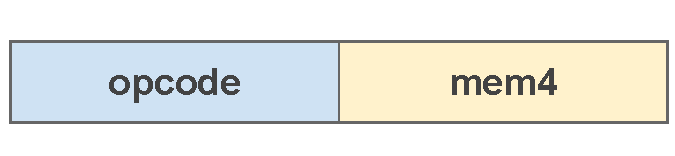
\includegraphics[width=0.47\textwidth]{figures/opcode}
	\centering
	\caption{8-bit instruction, 4-bit for opcode and 4-bit for memory operand.}
	\label{fig:opcode}
\end{figure}

Currently, we have only implemented 6 instructions, as shown below.

\begin{itemize}
	\item	NOP : No operation
	\item	LDA mem4 : Load memory into register A
	\item	ADD mem4 : Load memory then add it to register A
	\item	DISPLAY\_CFG : Send configuration data to 1602A LCD~\cite{1602a}
	\item	OUT : Send data to 1602A LCD
	\item	HLT : Halt
\end{itemize}

\subsection{Register}
The CPU has two general registers and one instruction register which are 8-bit. The MAR is 4-bit due to the memory space we have.

For 4-bit register, we use 74173 TTL logic module that provided by the FPGA software Quartus. 74713 is a 4-bit D-type register with 3-state outputs. For 8-bit register, we put two 74173 in parallel to form one 8-bit register, as shown in~\autoref{fig:8bitreg}.

\begin{figure}[th]
	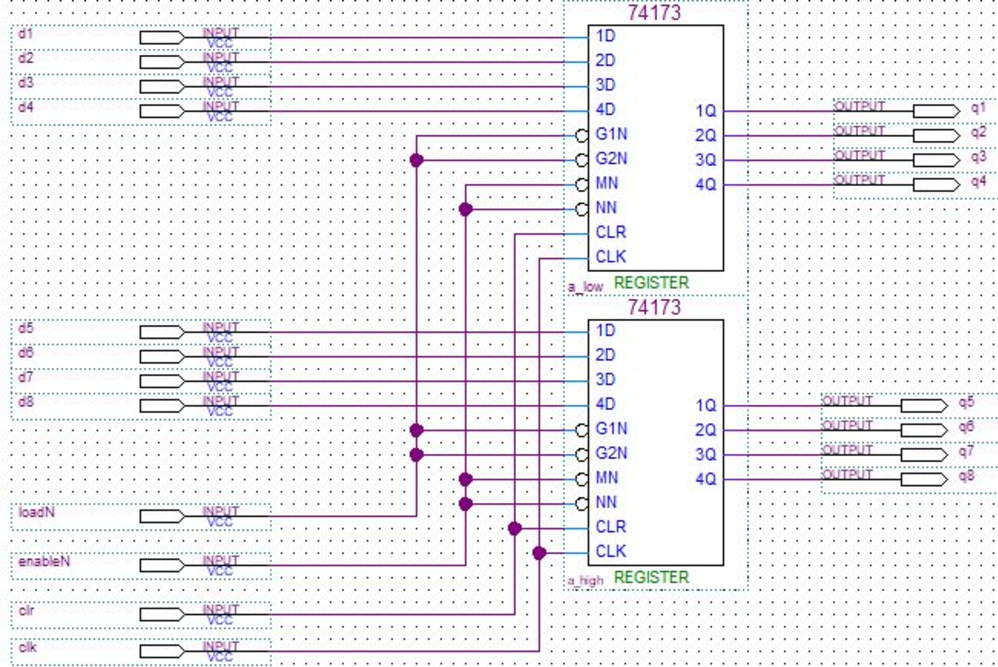
\includegraphics[width=0.47\textwidth]{figures/8bitreg}
	\centering
	\caption{8-bit register is composed of two 4-bit registers in parallel.}
	\label{fig:8bitreg}
\end{figure}


\subsection{MAR and Memory}

In this simple CPU, we do not use dynamic memory (DRAM) but static memory (SRAM). First, we are not sure whether FPGA can simulate capacitors and thus implement DRAM. Secondly, the CPU on modern computers runs much faster than memory, which requires a chipset to control it separately, or a CPU with a memory controller. We are not clear about these concepts yet, so we use SRAM to make memory and CPU work on the same frequency. This memory is quit similar to L1 instruction cache in modern computers, it only take one clock cycle to read/write. (Actually, because we use the memory module provided by Quartus, it takes 2 clock cycle to read/write. This is reflected in the control logic in our source code. But for simplicity, later in~\autoref{sec:casestudy}, we assume that the memory only takes one clock cycle to read/write data)


The memory address register either stores the memory address from which data will be fetched from the memory module, or the address to which data will be sent to store. Basically, MAR holds the memory location of data that needs to be accessed. Since the CPU only have 16 bytes memory space, the MAR only needs 4-bit. As shown in~\autoref{fig:marmem}, the MAR's input (d) connects to bus and it's output (q) connects to the memory module. There is only one signal for MAR. 
\begin{itemize}
	\item MI (MAR IN)
\end{itemize}
When it is signaled, the MAR loads 4-bit data from bus. There is no MAR OUT signal, which means MAR always output current value to the memory module.

\begin{figure}[th]
	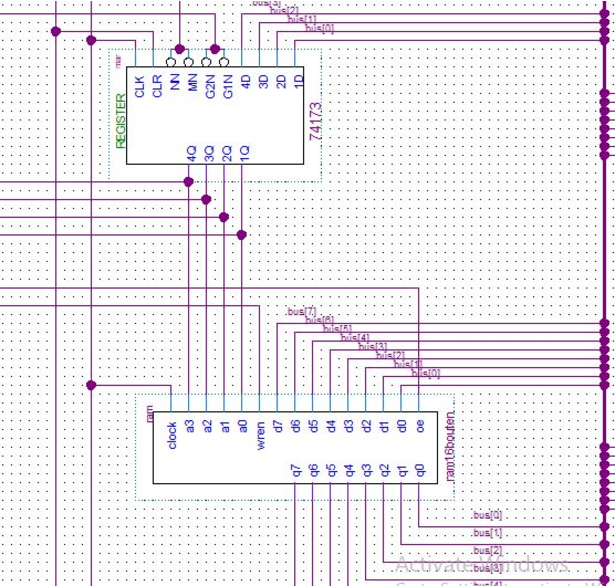
\includegraphics[width=0.47\textwidth]{figures/marmem}
	\centering
	\caption{MAR's input connects to bus and output connects to memory module.}
	\label{fig:marmem}
\end{figure}

The memory module's input (d) and output (q) are all connected with the bus. There are two control signals.

\begin{itemize}
	\item RI (RAM IN)
	\item RO (RAM OUT)
\end{itemize}

When RI is signaled, data will be sent to the memory. When RO is signaled, memory outputs data to the bus.


\subsection{IR}
IR is the register that holds the instruction being executed or decoded. Decoding the opcode in the instruction register includes determining the instruction, determining where its operands in memory, retrieving the operands from memory, allocating processor resources to execute the command, etc. In this case, as mentioned earlier, the low 4-bit is the only memory operand, so it will be output to the bus. The high 4-bit output of the IR is available to control logic, which generate the timing control signal that controls various processing components involved in executing the instruction. ~\autoref{fig:ir} shows that its input (d) connects to the bus, and its output (q) is divided into two parts, the low 4-bit part is sent to the bus, the high 4-bit part which is the opcode is sent to the control logic.

\begin{figure}[th]
	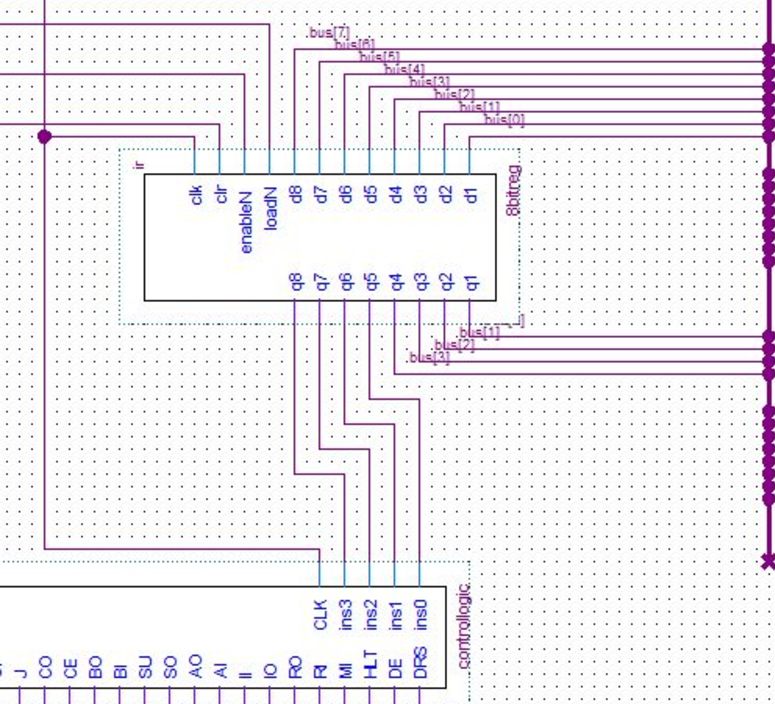
\includegraphics[width=0.47\textwidth]{figures/ir}
	\centering
	\caption{IR's input connects to bus and output to both bus and control logic.}
	\label{fig:ir}
\end{figure}

It has two control signals.

\begin{itemize}
	\item II (IR IN)
	\item IO (IR OUT)
\end{itemize}

II controls when the IR gets the instruction from the bus. When IO is signaled, IR outputs to both bus and control logic.


\subsection{General Registers}

We have two general registers A and B. As shown in~\autoref{fig:genreg}, they are both connected to ALU module. Although they are called general-purpose registers, register A is special, it's also an accumulator register. Because our instruction set design is too simple, no operand is used to indicate the register, so the default register for some instructions such as "ADD mem4" is register A.
 
\begin{figure}[th]
	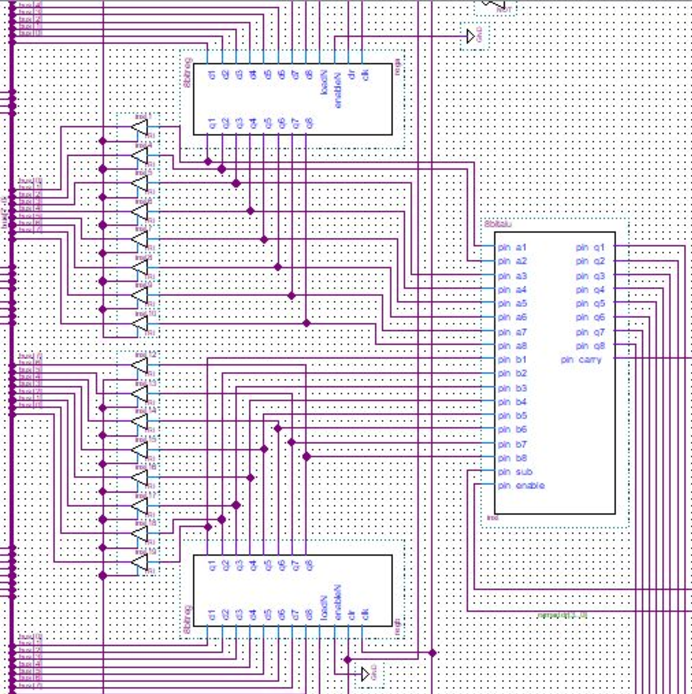
\includegraphics[width=0.47\textwidth]{figures/genreg}
	\centering
	\caption{Both general register A and B are connected to ALU and bus.}
	\label{fig:genreg}
\end{figure}

Each general register has two control signals, corresponding to the read and write of the register, as listed below.

\begin{itemize}
	\item AI (A IN)
	\item AO (A OUT)
	\item BI (B IN)
	\item BO (B OUT)
\end{itemize}



\subsection{PC}

The program counter (PC), commonly called the instruction pointer (IP) in Intel x86 microprocessors, and sometimes called the instruction address register (IAR) is a processor register that indicates where a CPU is in its program sequence.

Because our memory address space is only 16 bytes, the PC only needs 4 bits to cover the entire memory.

\begin{figure}[th]
	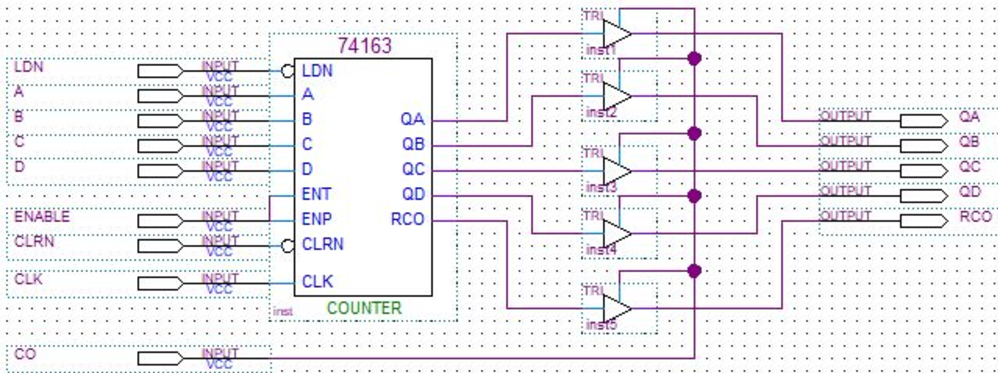
\includegraphics[width=0.47\textwidth]{figures/pc}
	\centering
	\caption{4-bit Program Counter}
	\label{fig:pc}
\end{figure}

We use 74163 4-bit counter as our program counter. Its 4-bit output will be sent to bus as a memory address to get one instruction from memory.

It also has two signals.

\begin{itemize}
	\item CE (COUNTER ENABLE)
	\item CO (COUNTER OUT)
\end{itemize}

When CO is signaled, the program counter output its content to the bus. Without CE signal, program counter will not increase on each clock cycle.


\subsection{Control Logic}

Their are 18 control signals in our design. The combination of signals can control the transmission of data between corresponding components. For example, issuing AO (A OUT) and BI (B IN) at the same clock cycle can make the data in register A transferred to register B. These signals can be regarded as atomic operations, and the function of control logic is to form a complete instruction through these operations.

Each instruction requires many clock cycles to complete, and several control signals need to be issued in each clock cycle. To do this, we use ROM to encode the instruction logics. Some instructions are more complicated and required more steps, and some instructions are relatively simple. So we set that each instruction needs to be completed in 6 steps. We use an 74163 4-bit counter to count the steps, as shown in~\autoref{fig:controllogic}.

\begin{figure}[th]
	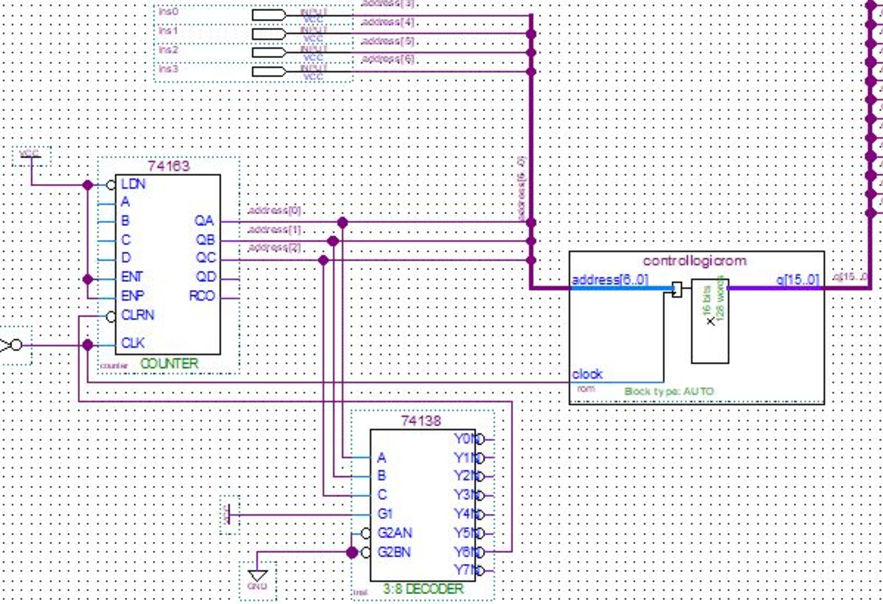
\includegraphics[width=0.47\textwidth]{figures/controllogic}
	\centering
	\caption{Control Logic Module}
	\label{fig:controllogic}
\end{figure}

The opcode of the instruction and each step number are encoded into an address. This address is used to index the data in the ROM. The data word width is 24 bits, which corresponds to 24 control signals. So far we have only used 18 of them.

%! TEX root = 'main.tex'
\section{Case Study}
\label{sec:casestudy}
In this section, we use an example to show how our CPU executes an instruction.
We designed a load instruction
\begin{lstlisting}
LDA mem4
\end{lstlisting}
This instruction indicates that the 4-bit operand is used as the memory address to read 1 byte of data into register A. For example, we want to load data from memory address 0xE, then the instruction is "LDA 0xE". Because the opcode of the LDA instruction is defined as 0x1, the binary form of this instruction is 0001 1110 (0x1E).

LDA instruction takes 4 clock cycle to finish.

\begin{enumerate}
	\item CO MI
	\item RO II CE
	\item IO MI
	\item RO AI
\end{enumerate}

In these four clock cycles, the first two can be regarded as the instruction fetch phase. These two cycles are the same in almost all the instructions we implemented.

Suppose the initial state of the CPU is as follows.

\begin{itemize}
	\item PC = 0x0
	\item Memory is initialized as in~\autoref{tab:memory}
\end{itemize}

\begin{table}[th]
	\begin{tabular}{|c|c|c|c|c|c|c|c|c|c|c|c|c|c|c|c|} 
		\hline
		0x0 & 0x1 & 0x2 & 0x3 & ...  & 0xB & 0xC & 0xD & 0xE & 0xF \\ 
		\hline
		0x1E & 0 & 0 & 0 & ... & 0 & 0 & 0 & 0xA & 0 \\
		\hline
	\end{tabular}
	\caption{Memory}
	\label{tab:memory}
\end{table}

The program counter points to the beginning of the memory, which stores the instruction binary 0x1E. At memory 0xE, which is the position to be read by this instruction, there is data 0xA.

\subsection{Clock Cycle 1}

We issue two control signals.

\begin{itemize}
	\item CO (COUNTER OUT)
	\item MI (MAR IN)
\end{itemize}


By issuing these two control signals, the PC sends its 4-bit value to the bus, and the MAR get the 4-bit value from the bus, as shown in~\autoref{fig:cc1}.

\begin{figure}[th]
	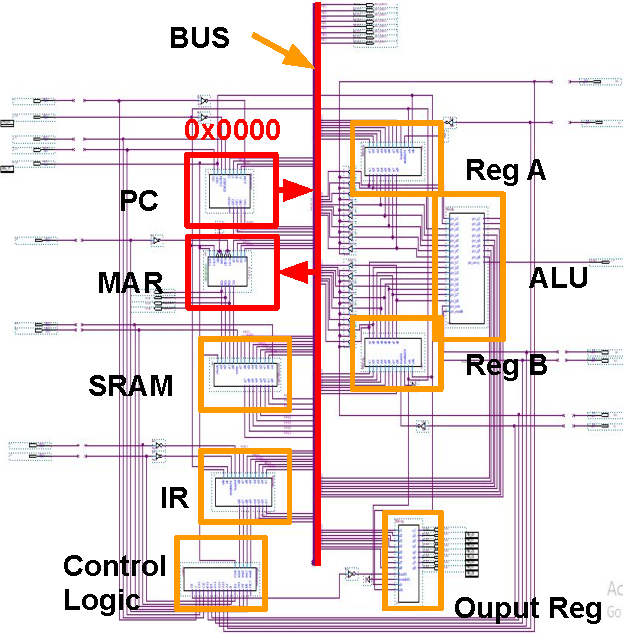
\includegraphics[width=0.47\textwidth]{figures/cc1}
	\centering
	\caption{Clock Cycle 1}
	\label{fig:cc1}
\end{figure}

As a result, the value in the PC is sent to the MAR and now MAR is 0x0.


\subsection{Clock Cycle 2}

We issue three control signals.

\begin{itemize}
	\item RO (RAM OUT)
	\item II (IR IN)
	\item CE (COUNTER ENALBE)
\end{itemize}

By issuing RO and II, the RAM sends the byte to the bus and the IR gets it, as shown in~\autoref{fig:cc2}. CE is also issued at this clock cycle, so the PC will increase one.

\begin{figure}[th]
	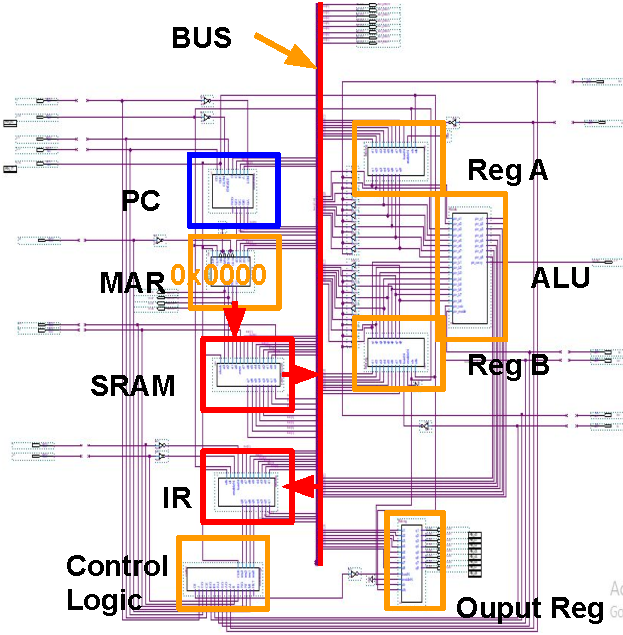
\includegraphics[width=0.47\textwidth]{figures/cc2}
	\centering
	\caption{Clock Cycle 2}
	\label{fig:cc2}
\end{figure}

As a result, the instruction is successfully loaded into the IR. Now IR contains value 0x1E.


\subsection{Clock Cycle 3}

We issue two control signals.

\begin{itemize}
	\item IO (IR OUT)
	\item MI (MAR IN)
\end{itemize}

This clock cycle can be viewed as the decoding phase. When IO is signaled, as mentioned earilier, the data in the IR is divided into two parts, the lower 4 bits are sent to the bus, and the upper 4 bits are send to the control logic, as shown in~\autoref{fig:cc3}.


\begin{figure}[th]
	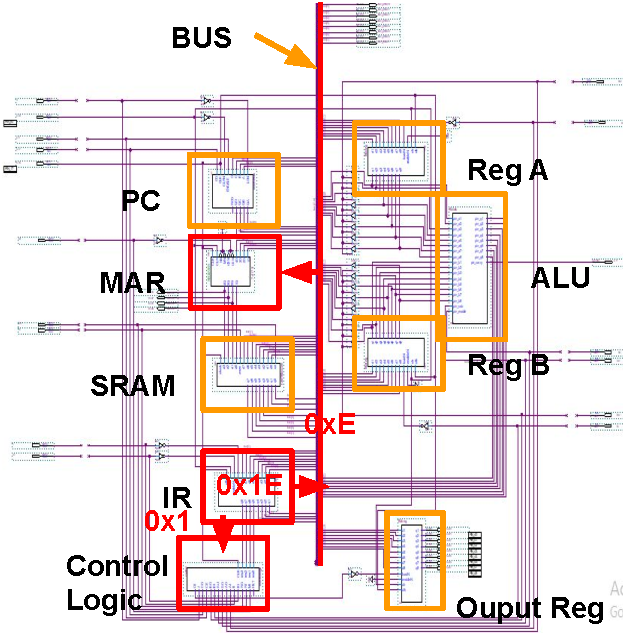
\includegraphics[width=0.47\textwidth]{figures/cc3}
	\centering
	\caption{Clock Cycle 3}
	\label{fig:cc3}
\end{figure}

As a result, the operand which is a memory address, now is loaded into MAR. MAR has 0xE and the control logic also gets the opcode.


\subsection{Clock Cycle 4}

We issue two control signals.

\begin{itemize}
	\item RO (RAM OUT)
	\item AI (A IN)
\end{itemize}

Because in the last clock cycle, the MAR already loaded with the memory address 0xE. In this clock cycle, the RO causes the memory to send the corresponding data to the bus. Meanwhile, register A gets data from the bus, as shown in~\autoref{fig:cc4}.

\begin{figure}[th]
	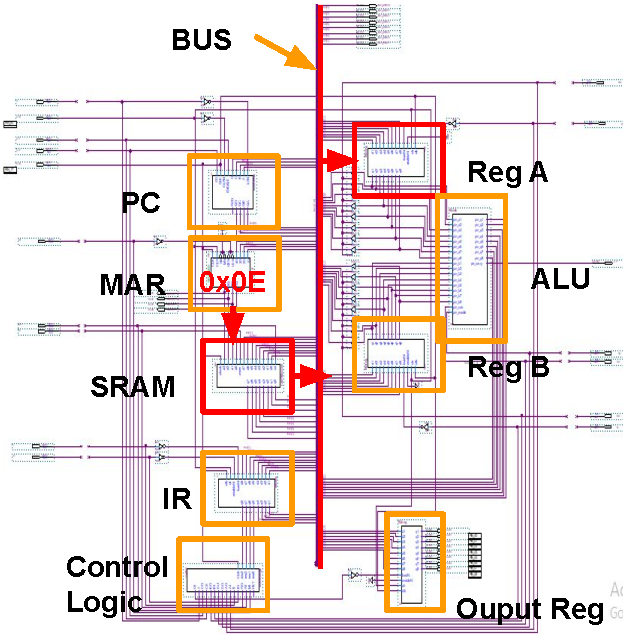
\includegraphics[width=0.47\textwidth]{figures/cc4}
	\centering
	\caption{Clock Cycle 4}
	\label{fig:cc4}
\end{figure}

So we see that when this clock cycle ends, the value in memory 0xE has been successfully loaded into register A. Now register A has the value 0xA.

%! TEX root = 'main.tex'
\section{System Setup}
\label{sec:setup}

\subsection{Source Code}

The source code of this 8-bit CPU is uploaded to Github~\footnote{https://github.com/whensungoesdown/8bitcpu}.

It has the following source code files.

8-bit register:
\begin{itemize}
	\item 8bitreg.bdf
	\item 8bitreg.bsf
\end{itemize}

8-bit ALU:
\begin{itemize}
	\item 8bitalu.bdf
	\item 8bitalu.bsf
\end{itemize}

Control Logic:
\begin{itemize}
	\item controllogic.bdf
	\item controllogic.bsf
	\item controllogicrom.bsf
	\item controllogicrom.cmp
	\item controllogicrom.mif
	\item controllogicrom.qip
	\item controllogicrom.vhd
\end{itemize}

4-bit counter:
\begin{itemize}
	\item counter4b.bdf
	\item counter4b.bsf
\end{itemize}

Memory:
\begin{itemize}
	\item ram16bouten.bdf
	\item ram16bouten.bsf
	\item ram16byte.bsf
	\item ram16byte.cmp
	\item ram16byte.qip
	\item ram16byte.vhd
	\item 16byteram.mif
\end{itemize}

Frequency divider:
\begin{itemize}
	\item clk1MHz.bsf
	\item clk\_div50.vhd
\end{itemize}


CPU assembly:
\begin{itemize}
	\item testcpu3.bdf
	\item testcpu3.qpf
	\item testcpu3.qsf
\end{itemize}

Waveform files for debugging purpose:
\begin{itemize}
	\item *.vwf
\end{itemize}


\subsection{Setup}
The FPGA developing board we use is Cyclone II~\cite{cyclone2} EP2C5 Mini Dev Board. And the software we use is Quartus II 64-bit Web Edition.

The display we use is 1602A LCD. The hardware setup is shown in~\autoref{fig:setup}.


\begin{figure}[th]
	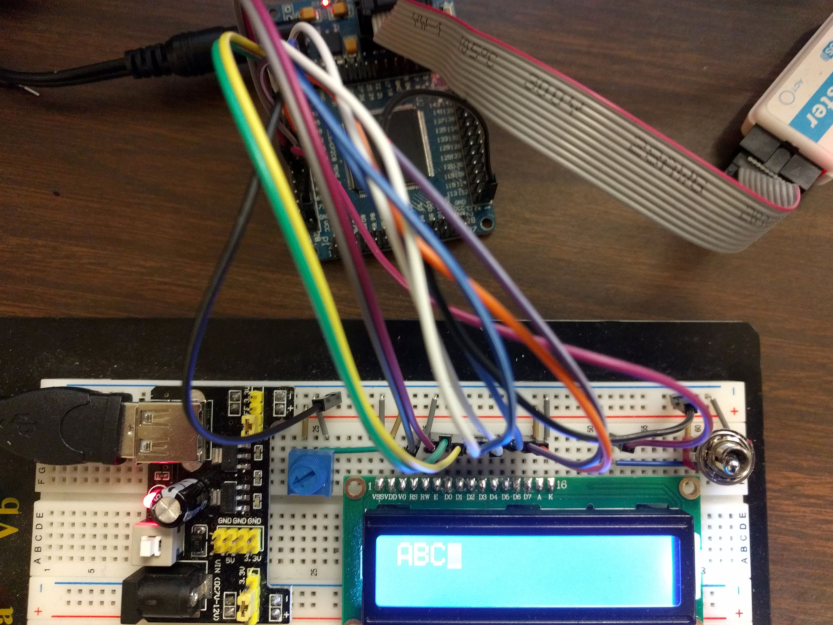
\includegraphics[width=0.47\textwidth]{figures/setup}
	\centering
	\caption{The CPU and display setup.}
	\label{fig:setup}
\end{figure}

We also need a USB Blaster to download the compiled code to the development board.

Both the Cyclone II development board and the LCD need 5V power supply. We power them separately with common ground. The FPGA's GPIO operating voltage is 3.3V. Because the LCD data pins have a wide range of operating voltage which accept 3.3V signals, we can directly connect the GPIO on the FPGA to the LCD. 

%%\input{sources/relatedwork}
%! TEX root = 'main.tex'
\section{Conclusions}
\label{sec:conclusions}
In this course project, we implemented a very simple 8-bit CPU on FPGA development board using simple TTL logic components such as the 74 series and very small amount of VHDL code. The CPU only has two general registers, and the ALU part can only do addition and subtraction. But it has some typical elements in CPU design such as IR, MAR, PC, memory and control logic. Through this course project, we understand better how a CPU executes an instruction. And have a more intuitive understanding of the bus.





\bibliographystyle{ACM-Reference-Format}
\bibliography{bib} 


%appendix
%%! TEX root = 'main.tex'
\appendix

\begin{appendices}

\section{}

\begin{lstlisting}[style=code]
library IEEE;
use IEEE.STD_LOGIC_1164.ALL;
use IEEE.numeric_std.all;

entity PatternOnWire is
	Port (CLK : in STD_LOGIC;
			Input: in STD_LOGIC;
			Output: out STD_LOGIC;
			LED : out STD_LOGIC);
end PatternOnWire;

architecture Behavioral of PatternOnWire is
	signal match : STD_LOGIC := '0';  --bool
	signal r_shift : STD_ULOGIC_VECTOR(7 downto 0);
begin	
	TmpP : process(CLK, Input)
		begin
		if CLK'event and CLK='1' then	 --rising edge
			r_shift(7) <= r_shift(6);
			r_shift(6) <= r_shift(5);
			r_shift(5) <= r_shift(4);
			r_shift(4) <= r_shift(3);
			r_shift(3) <= r_shift(2);
			r_shift(2) <= r_shift(1);
			r_shift(1) <= r_shift(0);
			r_shift(0) <= Input;
			
			if r_shift = "01010101" then
				match <= '1';
			else
				--match <= '0';
			end if;
			
		end if;
	end process;

	Output <= match;
	LED <= not(match);
end Behavioral;

\end{lstlisting}

\end{appendices}



\end{document}
